% Z-UO-BOOK -- The Triangular Lattice and Universal Optimality (student textbook)
% Sources: TOP20.json pick 8; papers/textbook_universal_optimality/{publication_meta.json,FACTS.md,editors_note.tex,
%          preface.tex}; results/discovery/D4/verification.md; memory note textbook-universal-optimality.md
% Figure: code/fig08.py -> figures/c08_disques.{pdf,png}
\chapter[Un manuel, un théorème]{Un manuel pour suivre un théorème jusqu'au laboratoire}
\reference{Publié le 11 octobre 2026.\\ doi:10.5281/\\zenodo.23295142}

\section*{L'idée en une image}

\begin{analogie}
Pensez à un livre de cuisine un peu particulier. Chaque recette y figure trois fois~: une explication pas à pas
(pourquoi ça marche), une analyse de laboratoire qui contrôle chaque ingrédient et chaque geste, et une dégustation.
Ici la \og recette\fg{} est un théorème~: l'explication est une preuve écrite pour un humain, l'analyse de
laboratoire est l'énoncé vérifié par le logiciel Lean, la dégustation est un test numérique en Python et en Rust.

\emph{Où l'image cesse d'être juste~:} l'analyse vérifie la recette par rapport à \emph{ses propres définitions},
pas qu'elle produit le plat que l'on voulait~; la dégustation ne dit que \og rien ne cloche dans les essais faits\fg~;
et l'ingrédient principal vient d'une autre cuisine, sans contrôle par des pairs.
\end{analogie}

\section*{Ce qui a été fait}

Ce manuel de 105 pages, destiné aux étudiants, suit un seul énoncé de ses définitions jusqu'au laboratoire~:
parmi toutes les façons de répartir des points dans le plan avec une densité donnée, l'arrangement en triangles
(celui des alvéoles d'une ruche, vu par leurs centres) a la plus petite énergie, pour toute une famille de
répulsions dites \og complètement monotones\fg{} (elles décroissent avec la distance d'une façon très régulière).
Ce théorème provient du dépôt public openai/math~; il a été produit par une IA et vérifié par le noyau de Lean.
Le manuel enseigne aussi tout ce qu'il faut pour le comprendre~: les
réseaux, la sommation de Poisson, les fonctions thêta, puis la physique où il apparaît, des tourbillons ponctuels
en mécanique des fluides aux réseaux de tourbillons d'un condensat, aux colloïdes, aux plasmas poussiéreux et aux
électrons sur l'hélium. Un dernier chapitre liste les questions ouvertes et des projets d'étudiants.

Les cinq chapitres ont été écrits chacun par un agent séparé, à partir d'une même fiche de faits imposée, puis
assemblés. Le premier relit un brouillon antérieur et y corrige huit erreurs, par exemple une confusion entre
\og dérivées de signes strictement alternés\fg{} et la vraie définition, qui autorise l'égalité.

\paragraph{Le résultat nouveau du livre.} Pour parler de densité dans un nuage infini, on compte les points dans un
disque de rayon $R$ et on divise par l'aire $\pi R^2$. Faut-il compter les points posés \emph{sur} le bord~? Le
livre démontre, vérifié par le noyau, que cela ne change ni la densité limite, ni l'énergie, ni la conclusion du
théorème.

\begin{encadre}
\textbf{À faire avec un crayon.} Dans le réseau triangulaire de densité un, chaque point a six plus
proches voisins, à la distance $a=\sqrt{2/\sqrt3}\approx1{,}0746$ (dans les coordonnées du livre, ce sont les six
couples $(j,k)$ avec $j^2+jk+k^2=1$~: $(1,0)$, $(0,1)$, $(-1,0)$, $(0,-1)$, $(1,-1)$, $(-1,1)$). Prenez un disque
centré sur un point, de rayon exactement~$a$, d'aire $\pi a^2=2\pi/\sqrt3\approx3{,}63$.
\begin{itemize}
\item Disque \emph{fermé} (bord compris)~: le centre et ses six voisins, soit $7$ points~; $7/3{,}63\approx1{,}93$.
\item Disque \emph{ouvert} (bord exclu)~: le centre seul, soit $1$ point~; $1/3{,}63\approx0{,}28$.
\end{itemize}
Pour un petit disque, la différence est énorme. Mais quand $R$ grandit, le bord ne pèse plus rien devant
l'intérieur, et les deux rapports tendent vers $1$ (figure~\ref{fig:c08}, à gauche). Le théorème transforme cette
intuition en preuve.
\end{encadre}

\begin{figure}[htbp]
\centering
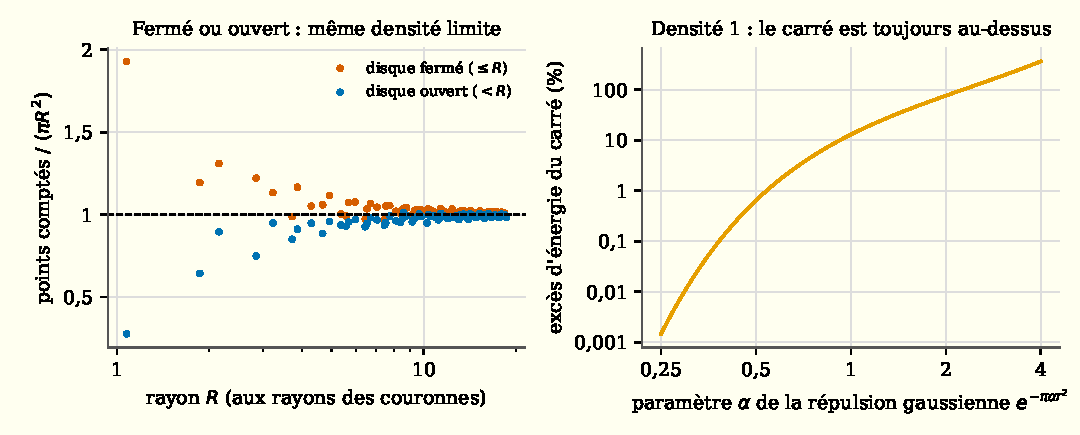
\includegraphics[width=\linewidth]{figures/c08_disques}
\caption{Densité comptée en disque fermé ou ouvert (gauche)~; excès d'énergie gaussienne du réseau carré (droite,
\niveau{X}).}
\label{fig:c08}
\end{figure}

\section*{Comment on s'est assuré que ce n'est pas faux}

En résumé~: \niveau{A} pour le résultat nouveau du livre (disques ouverts ou fermés), à densité un~; \niveau{C} aux
autres densités~; le théorème de départ est généré par une IA et n'a pas été relu par des pairs.

Pour le résultat sur les disques, \og le juge a regardé\fg~: le noyau de Lean, ce petit programme qui contrôle chaque pas
logique, l'a accepté, avec seulement trois axiomes standard. L'énoncé a été annoncé avant d'écrire la preuve. Un
vérificateur séparé, un agent d'IA distinct, l'a recompilé et a planté une fausse preuve, qui a été repérée. Il
a même trouvé mieux que prévu~: une des hypothèses (le nuage n'a qu'un nombre fini de points dans chaque disque)
est inutile, et il l'a démontré. Il a aussi vérifié, au noyau, que l'égalité n'est pas un tour de passe-passe des
définitions~: pour un seul point posé sur le cercle de rayon $1$, le disque ouvert en compte $0$ et le fermé $1$.
Ce sont les limites qui coïncident, pas les comptes. Le rejeu complet du 26 octobre 2026 a repassé ces deux modules
sans erreur.

Le livre entier a ensuite été audité par une autre instance de modèle d'IA~; aucun expert humain ne l'a relu.
Cet audit a donné 20 corrections, toutes appliquées, et les
scripts relancés ont donné les mêmes résultats. En l'écrivant, on a trouvé une erreur dans un article antérieur du
projet~: la simulation coupait le potentiel à une certaine distance, et, pour la portée la plus longue étudiée, cette
coupure déplaçait les énergies d'environ $1{,}8\times10^{-2}$, plus que l'écart entre réseau triangulaire et réseau carré. L'écart lui-même ne change
presque pas, mais la simulation portait sur une approximation sortie du cadre du théorème. Le livre publie cet
erratum.

\section*{Ce que ça ne dit pas}

\begin{limite}
\begin{itemize}
\item Le théorème de départ est généré par une IA et non relu par des pairs~; tout le livre en dépend.
\item Le résultat sur les disques vaut pour les quantités du théorème (disques centrés, énergie \og inférieure\fg)~;
  rien sur des fenêtres carrées ou de vraies conditions aux bords. Aux densités autres que un, il reste au niveau
  \niveau{C}.
\item La version forte de la conjecture (potentiel par potentiel) et le cas limite $s=2$ des potentiels en
  puissance restent ouverts, comme l'unicité parmi les configurations périodiques~; le livre le dit à chaque fois.
  En dimensions 8 et 24, le résultat analogue est démontré dans la littérature, mais pas formalisé ici~; en
  dimension 3, aucun arrangement universellement optimal n'est connu.
\item Le livre n'a pas de registre de revendications à lui.
\end{itemize}
\end{limite}

\section*{Pour aller plus loin}

Le manuel, ses sources \LaTeX, ses scripts et ses fichiers Lean sont déposés sous doi:10.5281/\allowbreak zenodo.23295142.
Une relecture critique par des étudiants, des enseignants ou des curieux y est explicitement invitée.
